\section{Introduction}\label{section:Intro}

The Large Underground Xenon (LUX) experiment has reported results from a WIMP dark matter 
search making use of its complete dataset. As reported in Ref.~\cite{Run4Paper}, no 
evidence for WIMP scattering events is found, and restrictive bounds on the allowed dark 
matter parameter space are derived.

The LUX WIMP target material is 250 active kg of liquefied xenon (LXe) 
instrumented as a dual phase time 
projection chamber (TPC). Scintillation light from ionizing events, known
as S1, is collected by arrays of photomultiplier tubes (PMTs) located above and below the liquid, 
while liberated charge from the event is collected by an anode located several centimeters above the liquid
surface. The anode region electric field is sufficient to generate secondary scintillation, known
as S2, from the charge deposit, which is also measured and localized in the $xy$ plane by the 
same PMT arrays. The $z$ coordinate of the event location is inferred
from the drift time between the S1 and S2 signals. A complete description of the detector is given in Ref.~\cite{nimpaper}. 

Background events in LUX typically result in electron recoil events, while the WIMPs are
expected primarily create nuclear recoils. In LXe these event types can be statistically distinguished by 
comparing the S1 and S2 signals of each event, since nuclear recoils create less
S2 than electron recoils for the same S1. The LUX WIMP search fits the S1 and S2 signals
of the WIMP search data to electron recoil and nuclear recoil models determined by tritium and neutron
calibration data.

LUX makes extensive use of an $^{83m}$Kr 
calibration source dissolved into the bulk of the LXe 
to monitor and correct for the detector response as a function of time and event position~\cite{scottspaper}.
The source is injected into LUX weekly, and it 
produces two sequential decays consisting of a mixture of internal transition electrons, x-rays, 
and Auger electrons, resulting in 32.1~keV and 9.4~keV electron-like energy deposits. 
The half-life of the 
intermediate state between the two energy deposits is 154~nanoseconds. 

Ref.~\cite{scottspaper}
describes how detector efficiency correction functions for the LUX 2013 WIMP search data (WS2013) are
derived from  $^{83m}$Kr calibration data. In general
the S1 signal depends on the event location due to the varying light collection efficiency, 
while the S2 signal depends on $z$ due to charge attenuation and on $xy$ due to 
anode gain variations. If the electric field is sufficiently uniform and constant, then any
variation in the S1 and S2 signals, summed over 
then the 32.1~keV and 9.4~keV decays, can be attributed to detector efficiency effects. The
electric field condition is approximately satisfied by the LUX TPC in 2013, and appropriate 
correction functions were derived from $^{83m}$Kr weekly calibration runs and applied to the 
WS2013 search data.


Data collected by LUX between 2014 and 2016 (WS2014-16) is substantially 
more complex than that of WS2013 because the TPC suffered from a highly non-uniform and slowly time-varying 
electric field during this period. The WS2014-16 electric field is described in detail in Ref.~\cite{luciespaper},
where we report on a COMSOL model that accurately describes the field 
in three dimensions as a function of time. The model was developed by comparing the observed
event locations in LUX $^{83m}$Kr calibration data to simulated drift trajectories from the model.

The S1 and S2 yields in LXe depend on the electric field because of its effect on 
the recombination probability. And owing to the non-uniform and time-varying electric field in WS2014-16, 
the electron recoil band in this data, and, to a lesser extent, the nuclear recoil band, 
depend on the event location and time. In the LUX WIMP search this complexity was managed
by dividing the detector into four slices in $z$ and four time periods. 16 electron recoil bands and 
16 nuclear recoil bands are determined for these detector conditions, and the data is compared
to expectations in each of the 16 datasets. 

In this paper we report on the derivation and application of detector efficiency correction functions
derived from $^{83m}$Kr calibration data that are tolerant to a non-uniform electric field. The 
correction functions so derived accurately characterize the light and charge collection efficiencies 
of the detector as a function of position and time, and are therefore 
appropriate to apply to all event types (electron recoil and nuclear recoil). We note
that these corrections functions do not attempt to describe or correct 
the genuine variation in the charge and light yields
that result from the electric field non-uniformity. In fact, charge and light yield corrections 
can not be made in WIMP search data even in principle, since these yields depend on the event type (electron
recoil and nuclear recoil), which is unknown on an event-by-event basis.

However, to derive the efficiency correction functions from weekly $^{83m}$Kr calibration data, 
it is necessary to first artificially modify each dataset to make the data appear as it would have if
the electric field had been uniform and constant in time. This data modification is possible in calibration data
because each event is known to be an electron recoil. Once this modification is made, the 
remaining S1 and S2 variations can be attributed to light and charge collection effects that will
affect contemporaneous WIMP search data in the same way. (We note if the $^{83m}$Kr calibration data
were not first altered to the uniform-field condition, then the correction functions that would be
derived would be inappropriate to WIMP search data, since it would contain electric field effects on charge and
light yield physics at 41.5~keV that does not hold true for 1-6~keVee WIMP search events.) 

For the LUX WS2014-16 data, we choose to alter the $^{83m}$Kr data to appear as it would in a 
uniform and constant field of XXX V/cm. This is the value of the electric field at the center of
LUX in September 2015. To carry out the field-flattening in $^{83m}$Kr data, we make use of an observable
that is present in each calibration dataset that 
has a one-to-one dependence on the local electric field in each three dimensional voxel
of the detector. That observable is S1a/S1b, the ratio of the S1 signal from the 32.1~keV and 9.4~keV
$^{83m}$Kr decay. We derive data alteration functions that relate how the charge and light yields
should be modified as a function of as S1a/S1b in order to reproduce how S1 and S2 would 
have appeared had the field been XXX V/cm.




dividethe detector 
into three dimensional voxels and measure







As in the 
WS2013 data, the time variation of the corrections is tracked through weekly injections of the 
$^{83m}$Kr calibration source.




We developed
To determine the appropriate weekly correction functions in the presence of the WS2014-16 electric
field required new methods to be develop;

Correction functions can be der from 
The derivation of the efficiency correction functions for the WS2014-16 







recently published a search for direct evidence of Weakly Interacting Massive Particles (WIMPs)~\ref{Run4Paper}.  The search was performed with a dual-phase (liquid and gas) xenon time projection chamber (TPC) containing 250 kg of liquid xenon in the active detector volume.  Recoil events were observed as prompt VUV photons from scintillation (S1), and as liberated electrons which were drifted to the liquid surface via an applied electric field (S2). 


As with all dual-phase TPCs, the S1 and S2 signals varied according to the vertex position of the interaction.  These signal variations resulted from both detector inefficiencies and field induced effects.  In the case of detector inefficiencies, the detection efficiency of S1 photons was roughly 30\% larger for events close to the cathode, when compared to those at the liquid surface. Similarly, loss of electrons to electronegativity impurities resulted in depth-dependent variation in the S2 signal, with 20-50\% of electrons liberated at the bottom of the detector reaching the liquid surface, depending on the purity of the liquid xenon at the time.  These sources of pulse area variations are independent of the energy of an event, or the type of recoil interaction that occurred, and can therefore be removed by applying event-agnostic position dependent signal corrections as was done in~\ref{Run3Reanalysis}.  Note that these energy and recoil-independent signal variations will be referred to as "detector inefficiencies" throughout this paper. 




As detailed in~\ref{Run4Paper}, the anode, gate, and cathode grids underwent a conditioning campaign inbetween LUX's WS2013 and WS2014–16 data collections.  This campaign increased the operating extraction field from 2.9 kV/cm to 3.5 kV/cm, and the detector's electron extraction efficiency from 49$\pm$3\% to 73$\pm$4\%.  After completing the grid conditioning campaign, deviations in the trajectory of free electrons, as well as inconsistencies in electron lifetime measurements across multiple sources, led to the conclusion that a non-uniform and time-varying negative
charge density in the polytetrafluoroethylene (PTFE)
panels had developed during the campaign.

The resulting nonuniform drift field introduced a second source of position dependent signal variations.  During a recoil event, ionizing radiation produces both ionization and excitation of the xenon atoms.  The xenon excimers (Xe$_2^*$) produce scintillation light as they return to the ground state, which we observe as our S1 signal. Some of the electrons produced during ionization escape the location of the event, drift to the top of our detector, and produce our S2 signal.  The electrons that do not escape the event recombine with the ionized xenon atoms in a process called recombination, producing additional xenon excimers that contribute to the S1 signal.  Recoil events which occur in a lower field region of the detector have a higher chance to recombine, and therefore produce more S1 signal and less S2 signal than an equivalent event in a high field region.  The strength of this effect is dependent on the energy of the event and whether the event is an electron recoil (ER) or a nuclear recoil (NR) (Figure \ref{fig:LYQY}).  Note that these energy and recoil-dependent signal variations will be referred to as "field effects" in this paper.  

\begin{center}
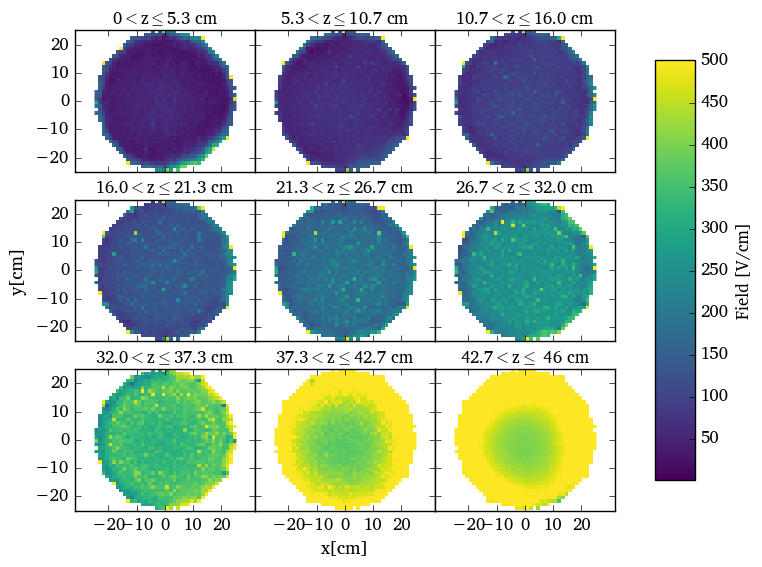
\includegraphics[scale=0.48]{figures/Fig1.png}
\captionof{figure}{LUX electric field map for September 2015, determined with a COMSOL\cite{comsol} electrostatic model compared drift trajectory data, as described in \cite{lucie}.}
 \label{fig:FieldMapExample}
\end{center}

%%%%%%%%%%%%%%%%%%%%%%%%
% Old Fig 1: Nest yields for light and charge
%%%%%%%%%%%%%%%%%%%%%%%
%\begin{center}
%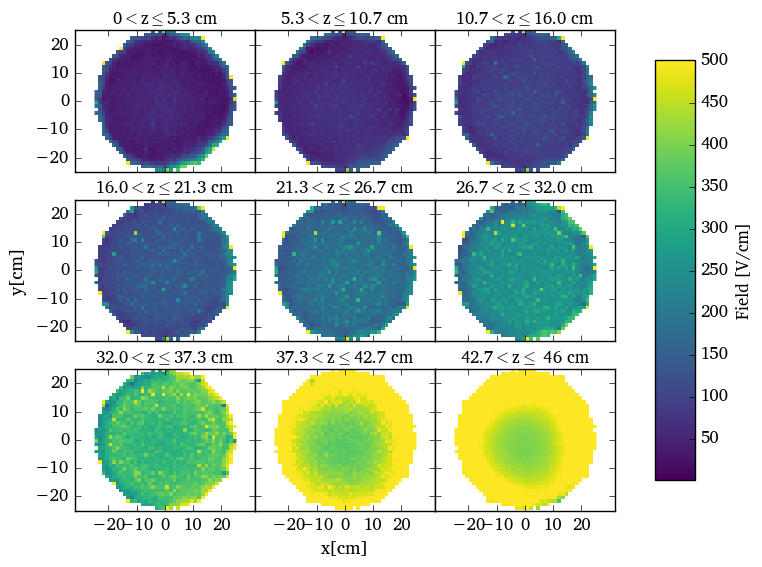
\includegraphics[scale=0.25]{figures/Fig1.png}
%\captionof{figure}{Predictions from NEST for the light yield (top row) and charge yield (bottom row) of electron recoil event from gamma ray interaction (left column) and beta particle interaction (right column).  Field values are indicated by the colored lines.  Light yield and charge yield have less dependence on the field strength for lower energy events.  \cite{RecombSource} }
%\label{fig:LYQY}
%\end{center}
